\chapter{Zadatak C} \label{ch:c}

U ovom poglavlju je opisan i odrađen zadatak C.

\section{Opis zadatka} \label{sec:c:opis}
odrediti fizikalnu sliku vozila prema matematičkom modelu s auditornih vježbi. Potrebno je prikazati
krivulje svake komponente sile zasebno i sve na jednom grafu s točno naznačenim oznakama.
Dodatno, za svaku komponentu sile je potrebno odrediti minimalnu, maksimalnu i srednju vrijednost
krivulje, te prikazati je u tabličnom obliku

\section{Rješenje} \label{sec:c:rjesenje}

Slika vozila sa svim silama koje djeluju na vozilo prikazana je na
slici~\ref{fig:c:forces}. Slika je kopirana iz prezentacije. Sila F\_a i F\_u su
sjedinjenje u jednu pošto akcelometar mjeri i ubrzanje i gravitaciju. Sila F\_k
računa se koristeći 'AccelerationZ' pošto je ta os okomuta na vozilo i cestu.
Sila F\_z računa se koristeći 'Velocity' i ostale konstante.
Konačna sila F je vektorski zbroj navedenih sila.


\begin{figure}
    \centering
    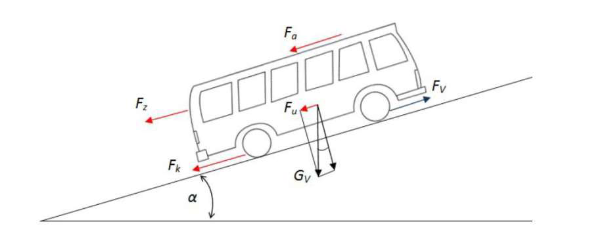
\includegraphics[width=0.8\textwidth]{images/vehicle.png}
    \caption{Prikaz svih sila koje djeluju na vozilo.}
    \label{fig:c:forces}
\end{figure}

\begin{figure}
    \centering
    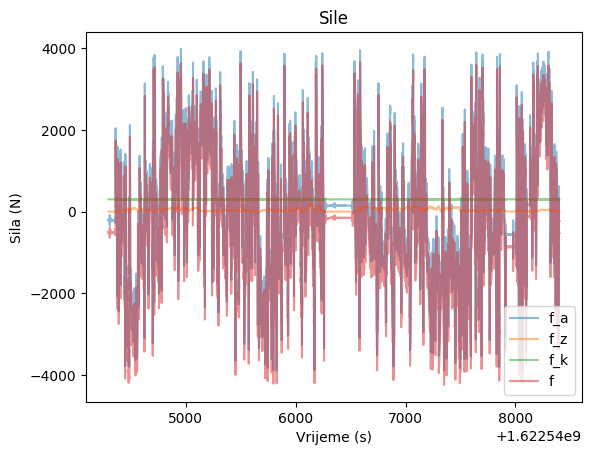
\includegraphics[width=0.8\textwidth]{images/forces.png}
    \caption{Prikaz izračunatih sila kroz vrijeme.}
    \label{fig:c:force_graph}
\end{figure}

\begin{table}[!ht]
    \centering
    \caption{Anaiza sila na vozilo}
    \begin{tabular}{lllll}
    \hline
        \textbf{describe} & \textbf{f\_a} & \textbf{f\_z} & \textbf{f\_k} & \textbf{f} \\ \hline
        count & 9776.0 & 9776.0 & 9776.0 & 9776.0 \\ 
        null\_count & 0.0 & 0.0 & 0.0 & 0.0 \\ 
        mean & 108.203167 & 40.246409 & 299.161135 & -231.204377 \\ 
        std & 1304.093637 & 38.85141 & 3.051616 & 1306.52905 \\ 
        min & -3895.112885 & 0.0 & 289.898032 & -4236.798241 \\ 
        25\% & -636.888744 & 0.355842 & 297.584225 & -973.533845 \\ 
        50\% & 146.215303 & 34.574766 & 299.567662 & -154.408851 \\ 
        75\% & 831.09496 & 67.626311 & 300.537012 & 478.256518 \\ 
        max & 3977.415058 & 188.240394 & 307.981613 & 3648.567624 \\ \hline
    \end{tabular}
    \label{table:c:forces}
\end{table}